\documentclass[10pt]{article}
\usepackage[utf8]{inputenc}
\usepackage[T1]{fontenc}
\usepackage{amsmath}
\usepackage{amsfonts}
\usepackage{amssymb}
\usepackage[version=4]{mhchem}
\usepackage{stmaryrd}
\usepackage{hyperref}
\hypersetup{colorlinks=true, linkcolor=blue, filecolor=magenta, urlcolor=cyan,}
\urlstyle{same}
\usepackage{graphicx}
\usepackage[export]{adjustbox}
\graphicspath{ {./images/} }

\title{Tracking control of vertical taking-off and landing vehicles with parametric uncertainty }


\author{Wenjie Dong $\odot$ | Md Nur-Adam Dony | Mohammad Rafat}
\date{}


\begin{document}
\maketitle
Department of Electrical and Computer Engineering, The University of Texas Rio Grande Valley, Edinburg, Texas, USA

\section{Correspondence}
Wenjie Dong, Department of Electrical and Computer Engineering, The University of Texas Rio Grande Valley, Edinburg, TX 78539.

Email: \href{mailto:wenjie.dong@utrgv.edu}{wenjie.dong@utrgv.edu}

\begin{abstract}
Summary This paper considers the position and attitude tracking control of a quadrotor with inertia parameter uncertainty. With the aid of the cascade structure of the dynamics of the system, an immersion and invariance observer is proposed to estimate the unknown mass of the system first. Secondly, a saturation controller is designed for the thrust force. Thirdly, a virtual controller is proposed for the angular velocity of the quadrotor with the aid of a nonlinear transform of the Euler angles. Finally, adaptive and robust controllers are proposed for the torque input of the quadrotor to deal with the unknown inertia moment of the system. Simulation results show the effectiveness of the proposed algorithms.
\end{abstract}

\section{K E Y W O R D S}
nonlinear system, quadrotor, saturation control, tracking control, uncertain system, VTOL

\section{1 | INTRODUCTION}
The control of vertical taking-off and landing (VTOL) unmanned aerial vehicles (UAVs) has been an active research area in the past decades due to its potential applications in the areas such as surveillance, search and rescue missions, monitoring, etc. A VTOL UAV has three degrees of freedom (DOF) for position and three DOF for orientation. It can fly to any position with a desired orientation. Moreover, VTOL UAVs can operate in cluttered environments and hover for a long time in air. However, a VTOL UAV is an underactuated system because it generally has four inputs. The underactuated nature makes control of a VTOL UAV a challenging problem.

The dynamics of a VTOL UAV can be considered as a cascaded system which includes a position control subsystem and an orientation control subsystem. With the aid of the featured cascade structure, a controller can be designed in two steps. In the first step, a virtual controller is designed such that the position of a VTOL UAV converges to its desired position. The problem considered in this step is called the position tracking control problem. In the second step, a controller is designed with the aid of the virtual controller in step 1 such that the position and the orientation of the VTOL UAV converge to its desired position and desired orientation, respectively. The problem considered in this step is called the attitude tracking problem. Based on the cascade structure, different controllers were proposed with the aid of backstepping techniques. ${ }^{1-5}$

In the controller design, the attitude of a VTOL UAV can be defined by its Euler angles or an unit quaternion. The controllers based on the Euler angles generally have singularities, while the controllers based on the quaternion generally have ambiguities in representing an attitude. To overcome these, the tracking controllers were designed directly on the special Euclidian group SE(3) ${ }^{6-8}$ In these results, there is an important assumption that the total thrust is nonzero. To make this assumption satisfied, it is generally assumed that the reference total thrust is bounded away from zero and the initial errors between the state of the system and the desired value of the state of the system are sufficiently small. Therefore, the controllers proposed in these papers are locally well-defined. In order to overcome this shortcoming, some researchers studied this problem and proposed well-defined controllers for large attraction region with the aid of saturation control. ${ }^{9,10}$ However, the tracking control of a VTOL UAV has not been studied if both the mass and the moment of a UAV are unknown.

In control of VTOL UAVs, there is always uncertainty in practice. Generally, there are two types of uncertainty. One type is called the parametric uncertainty which includes the unknown mass and inertia moment of a UAV. Another type of uncertainty is called the nonparametric uncertainty which includes unmodeled dynamics and disturbance. In order to deal with parametric uncertainty, several adaptive methods have been applied to design tracking controllers. In References 11 and 12, immersion and invariance technique was applied to design adaptive controllers. In Reference 13, adaptive backstepping technique was applied and an adaptive tracking controller was proposed. In Reference 14, adaptive tracking controllers were proposed without computation of derivatives of some signals with the aid of command-filter compensation. In these papers, the position tracking control problem was considered. However, both the position and attitude tracking control problem was not studied.

In this paper, we consider the position and attitude tracking control problem of a quadrotor with parametric uncertainty. An adaptive saturation controller is proposed with the aid of the backstepping technique, saturation control results, a nonlinear transformation of the Euler angles, and the immersion and invariance technique. If an estimation of the inertia parameter vector is known and the error between the estimate and the real value is upper bounded by a known constant, a robust controller is also proposed. The contributions of this paper are as follows:

\begin{enumerate}
  \item By introducing new saturation functions in the controller, the thrust force is guaranteed to be positive at any time.

  \item By a nonlinear transformation of the Euler angles, the singularity due to Euler angles is avoided during control. It is shown that in this paper the Euler angles will always be in the restrict regions if the initial Euler angles of the attitude are in the restrict regions.

  \item The proposed controllers can deal with the parametric uncertainty. Therefore, the proposed controllers can be applied to any quadrotors with different mass and inertia moments.

\end{enumerate}

This paper is organized as follows. In Section 2, the considered problem is defined and some preliminary results are presented. In Section 3, controllers are proposed to solve the defined problem with the aid of backstepping techniques. In Section 4, simulation is done to verify the proposed controllers. The last section concludes this paper.

\section{2 | PROBLEM STATEMENT AND SOME PRELIMINARY RESULTS}
\section{1 | Model of a quadrotor}
Let $\mathcal{F}: O-X Y Z$ be an earth fixed inertia frame. Its origin $O$ locates at a fixed point on the ground. $X$ axis points to north and $Z$ axis points upright. $Y$ axis is determined by the right hand. The unit vectors in the three axes are $e_{1}=[1,0,0]^{\top}$, $e_{2}=[0,1,0]^{\top}$, and $e_{3}=[0,0,1]^{\top}$, respectively. For a quadrotor, a body fixed frame $\mathcal{F}_{b}: O_{b}-X_{b} Y_{b} Z_{b}$ is rigidly attached to it. Its origin $O_{b}$ is located at the center of the mass of the quadrotor shown in Figure 1. Axes $X_{b}$ and $Y_{b}$ lie in the plane defined by the centers of the four rotors, as shown in Figure 1. The $Z_{b}$ axis is defined by the right hand. The coordinate of $O_{b}$ in the inertia frame is $p=[x, y, z]^{\top}$. Let $\Theta=[\varphi, \theta, \psi]^{\top}$ be the Euler angles of frame $\mathcal{F}_{b}$ with respect to frame $\mathcal{F}$, the attitude of the quadrotor is uniquely defined by $\Theta$. The attitude of the system can also be defined by the rotation matrix $R \in S O$ (3) from the inertia frame to the body frame

$$
R=\left[\begin{array}{ccc}
\mathrm{c} \theta \mathrm{c} \psi & \mathrm{s} \theta \mathrm{c} \psi \mathrm{s} \varphi-\mathrm{s} \psi \mathrm{c} \varphi & \mathrm{s} \theta \mathrm{c} \psi \mathrm{c} \varphi+\mathrm{s} \psi \mathrm{s} \varphi \\
\mathrm{c} \theta \mathrm{s} \psi & \mathrm{s} \theta \mathrm{s} \psi \mathrm{s} \varphi+\mathrm{c} \psi \mathrm{c} \varphi & \mathrm{s} \theta \mathrm{s} \psi \mathrm{c} \varphi-\mathrm{c} \psi \mathrm{s} \varphi \\
-\mathrm{s} \theta & \mathrm{c} \theta \mathrm{s} \varphi & \mathrm{c} \theta \mathrm{c} \varphi
\end{array}\right]
$$

F I G U RE 1 Configuration of a quadrotor

\begin{center}
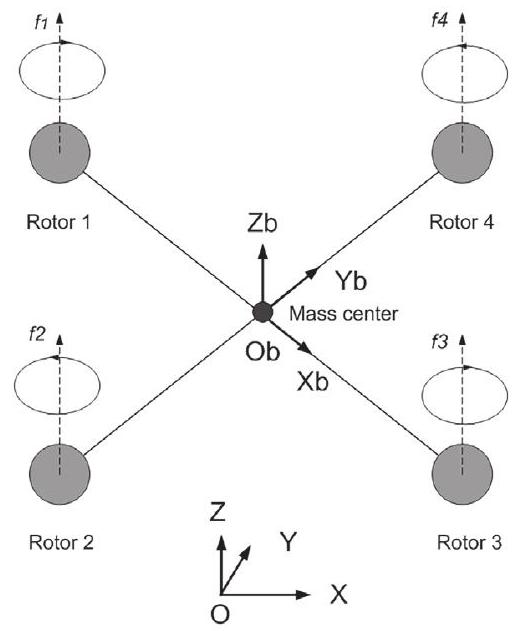
\includegraphics[max width=\textwidth]{2023_10_07_eefdf58cc80a47c1244eg-03}
\end{center}

where $c \theta$ denotes $\cos \theta$ and $\mathrm{s} \theta$ denotes $\sin \theta$. Under some assumptions, the kinematics and dynamics of the quadrotor are defined by

$$
\begin{gathered}
\dot{p}=v, \\
\dot{v}=-g e_{3}+\frac{1}{m} f R e_{3}, \\
\dot{R}=R S(\omega), \\
J \dot{\omega}=S(J \omega) \omega+\tau,
\end{gathered}
$$

where $g$ is the gravitational acceleration, $v$ is the velocity of the mass center in the inertia frame $\mathcal{F}, \omega=\left[\omega_{1}, \omega_{2}, \omega_{2}\right]^{\top}$ is the angular velocity of the quadrotor in the body frame $\mathcal{F}_{b}, J$ is the inertia matrix of the quadrotor, $S(\cdot)$ is a skew-symmetric matrix defined by

$$
S(\omega)=\left[\begin{array}{ccc}
0 & -\omega_{3} & \omega_{2} \\
\omega_{3} & 0 & -\omega_{1} \\
-\omega_{2} & \omega_{1} & 0
\end{array}\right],
$$

$f \in R$ is the total thrust produced by the four rotors along $Z_{b}$ axis, and $\tau=\left[\tau_{1}, \tau_{2}, \tau_{3}\right]^{\top}$ is the torque generated by the four rotors. In this paper, it is assumed that (i) the mass $m$ is an unknown constant and $m \in[\underline{m}, \bar{m}]$ where $\underline{m}$ and $\bar{m}$ are known constants; and (ii) the inertia matrix $J$ is an unknown constant matrix.

\section{2 | Problem statement}
In this paper, we consider the following tracking control problem.

Tracking Control Problem: It is given a desired trajectory $p^{d}(t)$ and a desired yaw angle $\psi^{d}(t)$, if the states $(p, v, \Theta, \omega)$ of the system is known and the inertia parameters $m$ and $J$ are unknown, the control problem is to design state feedback control inputs $f$ and $\tau$ such that

$$
\begin{aligned}
& \lim _{t \rightarrow \infty}\left(p(t)-p^{d}(t)\right)=0 . \\
& \lim _{t \rightarrow \infty}\left(\psi(t)-\psi^{d}(t)\right)=0 .
\end{aligned}
$$

For the desired trajectory, the following assumptions are made. Assumption 1. $p^{d}$ is smooth and $\left\|\ddot{p}^{d}\right\| \leq M_{d}$.

Assumption 2. $\psi^{d}$ is smooth. $\dot{\psi}^{d}$ and $\ddot{\psi}^{d}$ are bounded.

For the system, the following assumption is also made.

Assumption 3. The state $(p, v, \Theta, \omega)$ is measurable and is available for the controller design.

The above control problem is challenging. First, the system (2), (3), (4), (5) is an underactuated system. The number of the control inputs is less than the number of the DOF of the system. Fortunately, in the control problem there are four variables to be controlled. Secondly, the position control of the system is coupled to the attitude control. It is impossible to decouple (2), (3), (4), (5) into two independent subsystems. In order to deal with this, a modified backstepping technique will be applied. Thirdly, the mapping from the attitude to the Euler angles/the rotation matrix is not one-to-one. There are many research results on this problem in literature. In this paper, Euler angles are used to define the attitude. To make the mapping from the attitude to the Euler angles one-to-one, we restrict the Euler angles to the following regions:

$$
\varphi \in\left(\frac{-\pi}{2}, \frac{\pi}{2}\right), \theta \in\left(-\frac{\pi}{2}, \frac{\pi}{2}\right), \psi \in(-\pi, \pi)
$$

In practice, these regions are enough for flying a quadrotor. In this paper, controllers will be designed with the aid of a nonlinear transformation such that the Euler angles are within the above regions during all time if their initial conditions are within the above regions. Finally, there is uncertainty in the system which makes our control problem more challenging.

\section{3 | Some preliminary results}
Some results on saturation control will be applied in this paper. They are presented here.

Definition 1. (15) Given two positive constants $M$ and $L(L \leq M)$, a function $\sigma: R \rightarrow R$ is said to be a smooth linear saturation for $(L, M)$ if it is a smooth function satisfying

(a) $s \sigma(s)>0$ for all $s \neq 0$;

(b) $\sigma(s)=s$ if $|s| \leq L$;

(c) $|\sigma(s)| \leq M$ for all $s \in R$.

Lemma 1. Consider a system

$$
\dot{x}_{1}=x_{2}, \quad \dot{x}_{2}=u+d,
$$

where $d$ is bounded and asymptotically converges to zero, the control law

$$
u=-\sigma_{2}\left(k_{2} x_{2}+\sigma_{1}\left(k_{1} k_{2} x_{1}+k_{1} x_{2}\right)\right)
$$

ensures that $x_{1}$ and $x_{2}$ converge to zero, where the control parameters $k_{1}>0$ and $k_{2}>0, \sigma_{i}$ is a smooth saturation function for $\left(L_{i}, M_{i}\right)(i=1,2)$ and $M_{1}<L_{2} / 2, L_{1} \geq L_{2} / 2-M_{1}$. Furthermore, if $d$ exponentially converges to zero, after a finite time $x=\left[x_{1}, x_{2}\right]^{\top}$ exponentially converges to zero.

The lemma can be proved with the aid of the proof in ${ }^{15}$ and is omitted.

If $s=\left[s_{1}, \ldots, s_{m}\right]^{\top}$, we denote $\sigma(s)=\left[\sigma\left(s_{1}\right), \ldots, \sigma\left(s_{m}\right)\right]^{\top} . \mathcal{L}_{2}$ denotes the function space where each function is square-integrable (ie, $\int_{0}^{\infty} f^{2}(t) d t<\infty$ ) and $\mathcal{L}_{\infty}$ denotes the function space where each function is bounded (ie, $\sum_{t \geq 0}|f(t)|<$ $\infty)$. If $x \in \mathcal{L}_{2} \cap \mathcal{L}_{\infty}$, then $x$ is bounded and converges to zero by Barbalat's lemma.

\section{3 | CONTROLLER DESIGN}
By simple algebraic calculation, (4) can be written as

$$
\dot{\Theta}=W(\Theta) \omega,
$$

where

$$
W(\Theta)=\frac{1}{\cos \theta}\left[\begin{array}{ccc}
\cos \theta & \sin \varphi \sin \theta & \cos \varphi \sin \theta \\
0 & \cos \varphi \cos \theta & -\sin \varphi \cos \theta \\
0 & \sin \varphi & \cos \varphi
\end{array}\right]
$$

and $\operatorname{det}(W(\Theta))=\frac{1}{\cos \theta}$. W is nonsingular if $\theta \neq \frac{(2 k-1) \pi}{2}$ for any integer $k$. Our controller will be designed based on Equations (2), (3), (9), and (5).

Considering the structure of the system in (2), (3), (4), (5) and the requirements (8) on the Euler angles, a modified backstepping approach will be proposed in the controller design. It includes the following steps:

Step 1: Let $e_{p}=p-p^{d}$ and $e_{v}=v-\dot{p}^{d}$, we have

$$
\begin{gathered}
\dot{e}_{p}=e_{v} . \\
\dot{e}_{v}=\frac{1}{m} f R e_{3}-g e_{3}-\ddot{p}^{d} .
\end{gathered}
$$

Since $m$ is unknown, we estimate $\frac{1}{m}$ by an adaptive law. Let

$$
e_{m}=\beta+k_{m} e_{v}^{\top} R e_{3}-\frac{1}{m}
$$

where $k_{m}$ is a positive constant and $\beta$ is an estimation of $1 / m$, then

$$
\begin{aligned}
\dot{e}_{m} & =\dot{\beta}+k_{m} \dot{e}_{v}^{\top} R e_{3}+k_{m} e_{v}^{\top} R S(\omega) e_{3} \\
& =-k_{m} f e_{m}+k_{m} f\left(\beta+k_{m} e_{v}^{\top} R e_{3}\right)+\dot{\beta}-k_{m}\left(g e_{3}+\ddot{p}^{d}\right)^{\top} R e_{3}+k_{m} e_{v}^{\top} R S(\omega) e_{3} .
\end{aligned}
$$

The adaptive law of $\beta$ is chosen as

$$
\dot{\beta}=-k_{m} f\left(\beta+k_{m} e_{v}^{\top} R e_{3}\right)+k_{m}\left(g e_{3}+\ddot{p}^{d}\right)^{\top} R e_{3}-k_{m} e_{v}^{\top} R S(\omega) e_{3} .
$$

Then,

$$
\dot{e}_{m}=-k_{m} f e_{m},
$$

and

$$
e_{m}(t)=e_{m}(0) e^{-k_{m} \int_{0}^{t} f(\tau) d \tau}
$$

which means that $\left|e_{m}\right|$ does not increase if $f>0$. Furthermore, we have the following results.

Lemma 2. If $f>0$ and $\beta(0)$ and $k_{m}$ are chosen such that

$$
\beta(0) \geq k_{m}\left\|e_{v}(0)\right\|+\frac{1}{\underline{m}},
$$

then $e_{m}(t) \geq 0$ and exponentially converges to zero, which means that $\beta+k_{m} e_{v}^{\top} R e_{3}>0$ and exponentially converge to $\frac{1}{m}$.

Proof. By (15), $e_{m}(0)>0$. By (14), $e_{m}(t)>0$ and exponentially converges to zero if $f>0$. So, $\beta+k_{m} e_{v}^{\top} R e_{3}=e_{m}+\frac{1}{m}>0$ for any time and exponentially converge to $\frac{1}{m}$.

In the next steps, we will design a control law $f$ such that $f>0$ at any time.

Step 2: Consider $f R e_{3}$ as a virtual control input, we choose it such that (6) is satisfied. With the aid of the results in Lemma 1, we choose the virtual control input for $f R e_{3}$ as

$$
\alpha=\left[\begin{array}{l}
\alpha_{1} \\
\alpha_{2} \\
\alpha_{3}
\end{array}\right]=\frac{1}{\beta(t)+k_{m} e_{v}^{\top}(t) R(t) e_{3}}\left[g e_{3}+\ddot{p}_{d}-\sigma_{2}\left(k_{v} e_{v}+\sigma_{1}\left(k_{v} k_{p} e_{p}+k_{p} e_{v}\right)\right)\right],
$$

where $k_{p}$ and $k_{v}$ are positive constants, $\sigma_{i}$ is a smooth saturation function with parameter $\left(L_{i}, M_{i}\right)$ defined in the last section, and $L_{1}>L_{2} / 2-M_{1}>0$.

For the virtual control $\alpha$, we have the following results.

Lemma 3. For $\alpha$ defined in (16), if (15) holds and

$$
M_{2}<g-M_{d},
$$

then

$$
\alpha_{3}>0, \quad 0<\|\alpha(t)\| \leq c_{1}, \quad \forall t
$$

where

$$
c_{1}=\frac{g+M_{d}+M_{2}}{e_{m}(0)+1 / m} \text {. }
$$

Proof. By Lemma $2, \beta+k_{m} e_{v}^{\top} R e_{3}>0$. So, $\alpha$ is well defined. Noting that

$$
g+\ddot{p}_{d}(3)-\sigma_{M}\left(k_{v} e_{v}(3)+k_{p} e_{p}(3)\right) \geq g-M_{d}-M_{2}>0,
$$

where $e_{v}(3)$ means the third element of vector $e_{v}, \alpha_{3}>0$. So, $\|\alpha\|>0$. The boundedness of $\|\alpha\|$ is obvious since $1 /(\beta+$ $\left.k_{m} e_{v}^{\top} R e_{3}\right), \ddot{p}_{d}$, and $\sigma_{i}(\cdot)$ are all bounded.

With the aid of the virtual control $\alpha,(11)$ can be written as

$$
\dot{e}_{v}=-\sigma_{2}\left(k_{v} e_{v}+\sigma_{1}\left(k_{v} k_{p} e_{p}+k_{p} e_{v}\right)\right)-e_{m} \alpha+\frac{1}{m}\left(f R e_{3}-\alpha\right) .
$$

Step 3: In this step, we find $f$ and virtual control inputs $\varphi_{d}$ and $\theta_{d}$ for $\varphi$ and $\theta$. We choose

$$
f=\|\alpha\|
$$

Let $f e_{3}=R^{\top}\left(\Theta_{d}\right) \alpha$, simple calculation gives

$$
\begin{gathered}
\alpha_{1} \mathrm{c} \theta_{d} \mathrm{c} \psi_{d}+\alpha_{2} \mathrm{c} \theta_{d} \mathrm{~s}_{d} \psi_{d}-\alpha_{3} \mathrm{~s} \theta_{d}=0, \\
\alpha_{1}\left(\mathrm{~s} \theta_{d} \mathrm{c} \psi_{d} \mathrm{~s} \varphi_{d}-\mathrm{s} \psi_{d} \mathrm{c} \varphi_{d}\right)+\alpha_{2}\left(\mathrm{~s} \theta_{d} \mathrm{~s} \psi_{d} \mathrm{~s} \varphi_{d}+\mathrm{c} \psi \mathrm{c} \varphi_{d}\right)+\alpha_{3} \mathrm{c} \theta_{d} \mathrm{~s} \varphi_{d}=0, \\
\alpha_{1}\left(\mathrm{~s} \theta_{d} \mathrm{c} \psi_{d} \mathrm{c} \varphi_{d}+\mathrm{s} \psi_{d} \mathrm{~s} \varphi_{d}\right)+\alpha_{2}\left(\mathrm{~s} \theta_{d} \mathrm{~s} \psi_{d} \mathrm{c} \varphi_{d}-\mathrm{c} \psi_{d} \mathrm{~s} \varphi_{d}\right)+\alpha_{3} \mathrm{c} \theta_{d} \mathrm{c} \varphi_{d}=f,
\end{gathered}
$$

where $c \theta_{d}=\cos \theta_{d}$ and $s \theta_{d}=\sin \theta_{d}$. From (21) we have

$$
\theta_{d}=\arctan \left(\frac{\alpha_{1} \cos \psi_{d}+\alpha_{2} \sin \psi_{d}}{\alpha_{3}}\right) .
$$

The difference of Equation (23) multiplying $\sin \varphi_{d}$ and Equation (22) multiplying $\cos \varphi_{d}$ yields

$$
f \sin \varphi_{d}=\alpha_{1} \sin \psi_{d}-\alpha_{2} \cos \psi_{d}
$$

From this equation, we choose

$$
\varphi_{d}=\arcsin \left(\frac{\alpha_{1} \sin \psi_{d}-\alpha_{2} \cos \psi_{d}}{\|\alpha\|}\right)
$$

With the aid of the virtual control inputs $\varphi_{d}$ and $\psi_{d},(19)$ can be written as

$$
\dot{e}_{v}=-\sigma_{2}\left(k_{v} e_{v}+\sigma_{1}\left(k_{v} k_{p} e_{p}+k_{p} e_{v}\right)\right)-e_{m} \alpha+\frac{\|\alpha\|}{m} R\left(\Theta_{d}\right)\left(R\left(\Theta-\Theta_{d}\right)-I_{3}\right) e_{3} .
$$

Step 4: In this step, we design the virtual control for $\omega$ such that (6) and (7) are satisfied and the Euler angles $(\varphi, \theta, \psi)$ are in the restrict regions in (8). Let

$$
\xi=\left[\begin{array}{c}
\tan \varphi-\tan \varphi_{d} \\
\tan \theta-\tan \theta_{d} \\
\tan \frac{\psi}{2}-\tan \frac{\psi_{d}}{2}
\end{array}\right],
$$

then,

$$
\dot{\xi}=G(\Theta) W(\Theta) \omega-G\left(\Theta_{d}\right) \dot{\Theta}_{d}
$$

where

$$
G(\Theta)=\operatorname{diag}\left(\left[\frac{1}{\cos ^{2} \varphi}, \frac{1}{\cos ^{2} \theta}, \frac{1}{2 \cos ^{2} \frac{\psi}{2}}\right]\right) .
$$

It is obvious that $\Theta$ is in the regions in (8) and (7) holds if $\xi$ is bounded and converges to zero. To design a virtual controller for $\omega$, we choose a Lyapunov function

$$
V_{3}=\frac{1}{2} \xi^{\top} \xi
$$

Then,

$$
\dot{V}_{3}=\xi^{\top}\left(G(\Theta) W(\Theta) \omega-G\left(\Theta_{d}\right) \dot{\Theta}_{d}\right) .
$$

Choose the virtual controller of $\omega$ as

$$
\eta=(G(\Theta) W(\Theta))^{-1}\left(-k_{\Theta} \xi+G\left(\Theta_{d}\right) \dot{\Theta}_{d}\right)
$$

where $k_{\Theta}$ is a diagonal positive definite matrix. If $\omega=\eta$,

$$
\dot{V}_{3}=-\xi^{\top} k_{\Theta} \xi \leq 0,
$$

which means that $\xi$ exponentially converges to zero.

In (29), the inverse of $G(\Theta) W(\Theta)$ always exists because $\Theta$ is in the regions defined in (8) with the controllers defined in the next step.

Step 5: Since $\omega$ is not a real control input and cannot be $\eta$, we let

$$
\tilde{\omega}=\omega-\eta .
$$

Then,

$$
\begin{gathered}
\dot{\xi}=-k_{\Theta} \xi+G(\Theta) W(\Theta) \widetilde{\omega} \\
J \dot{\tilde{\omega}}=S(J \omega) \omega+\tau-J \dot{\eta} .
\end{gathered}
$$

Denote

$$
J=\left[\begin{array}{ccc}
J_{11} & J_{12} & J_{13} \\
J_{12} & J_{22} & J_{23} \\
J_{13} & J_{23} & J_{33}
\end{array}\right]
$$

and for any vector $\zeta=\left[\zeta_{1}, \zeta_{2}, \zeta_{3}\right]^{\top} \in R^{3}$ we define an operator

$$
\Gamma(\zeta)=\left[\begin{array}{cccccc}
\zeta_{1} & \zeta_{2} & \zeta_{3} & 0 & 0 & 0 \\
0 & \zeta_{1} & 0 & \zeta_{2} & \zeta_{3} & 0 \\
0 & 0 & \zeta_{1} & 0 & \zeta_{2} & \zeta_{3}
\end{array}\right],
$$

then

$$
J \zeta=\Gamma(\zeta) a
$$

where $a=\left[J_{11}, J_{12}, J_{13}, J_{22}, J_{23}, J_{33}\right]^{\top}$ is a collection of all elements of $J$. Equation (31) can be written as

$$
J \dot{\tilde{\omega}}=\tau-[S(\omega) \Gamma(\omega)+\Gamma(\dot{\eta})] a .
$$

Since $a$ is unknown, an adaptive control law will be proposed such that (6) and (7) are satisfied. To this end, we choose a Lyapunov function

$$
V_{4}=V_{3}+\frac{1}{2} \tilde{\omega}^{\top} J \tilde{\omega}+\frac{1}{2}(a-\hat{a})^{\top} \gamma^{-1}(a-\hat{a})
$$

where $\gamma$ is a positive definite constant matrix and $\hat{a}$ is an estimate of $a$ and will be designed later. The derivative of $V_{4}$ along the solution of (30) and (32) is

$$
\begin{aligned}
\dot{V}_{4} & =-\xi^{\top} k_{\Theta} \xi+\xi^{\top} G(\Theta) W(\Theta) \tilde{\omega}+\tilde{\omega}^{\top} \tau \\
& -\tilde{\omega}^{\top}[S(\omega) \Gamma(\omega)+\Gamma(\dot{\eta})] a-(a-\hat{a})^{\top} \gamma^{-1} \dot{\hat{a}}
\end{aligned}
$$

We choose the control law and the update law as follows:

$$
\begin{gathered}
\tau=-k_{\omega} \tilde{\omega}-[G(\Theta) W(\Theta)]^{\top} \xi+[S(\omega) \Gamma(\omega)+\Gamma(\dot{\eta})] \hat{a} . \\
\dot{\hat{a}}=-\gamma[S(\omega) \Gamma(\omega)+\Gamma(\dot{\eta})]^{\top} \tilde{\omega} .
\end{gathered}
$$

Then,

$$
\dot{V}_{4}=-\xi^{\top} k_{\Theta} \xi-\tilde{\omega}^{\top} k_{\omega} \tilde{\omega} \leq 0,
$$

which means that $\xi$ and $\tilde{\omega}$ converges to zero and $\hat{a}$ is bounded.

Based on the above controller design procedure, we have the following results.

Lemma 4. With the control input (33) and (34), (7) holds. Furthermore, $\Theta-\Theta_{d}$ converges to zero.

Proof. By the Lyapunov function $V_{4}$, we have (35), which means that $V_{4}$ is bounded, $\xi \in \mathcal{L}_{2}$, and $\tilde{w} \in \mathcal{L}_{2}$. The boundedness of $V_{4}$ means that $\xi, \tilde{\omega} \in \mathcal{L}_{\infty}$. So, $\xi$ and $\tilde{\omega}$ converge to zero, respectively. Therefore, (7) holds because the transformation $\tan (\cdot)$ is one-to-one mapping for angles in $(-\pi / 2, \pi / 2)$.

By the mean value theorem, we have

$$
\tan \varphi-\tan \varphi_{d}=\frac{1}{\cos \varphi_{c}}\left(\varphi-\varphi_{d}\right)
$$

where $\varphi_{c}$ is a value between $\varphi$ and $\varphi_{d}$. Since $\varphi, \varphi_{d} \in(-\pi / 2, \pi / 2), \frac{1}{\cos ^{2} \varphi_{c}} \leq c_{\varphi}$ where $c_{\varphi}$ is a positive constant. Since $\xi \in \mathcal{L}_{2}$, $\varphi-\varphi_{d} \in \mathcal{L}_{2}$. Similarly, it can be proved that $\theta-\theta_{d} \in \mathcal{L}_{2}$ and $\psi-\psi_{d} \in \mathcal{L}_{2}$. Therefore, $\Theta-\Theta_{d} \in \mathcal{L}_{2} \cap \mathcal{L}_{\infty}$. So, $\Theta-\Theta_{d}$ converges to zero.

Theorem 1. For the system in (2), (3), (4), (5) and a given desired trajectory ( $\left.p_{d}, \psi_{d}\right)$, under Assumptions 1, 2, 3, the control inputs $(f, \tau)$ in (20) and (33) with the update laws in (12) and (34) ensure that (6)-(7) are satisfied and $\hat{a}$ is bounded.

Proof. By Lemma 4, (7) holds and $\Theta-\Theta_{d}$ converges to zero. Let

$$
d=-e_{m} \alpha+\frac{\|\alpha\|}{m} R\left(\Theta_{d}\right)\left(R\left(\Theta-\Theta_{d}\right)-I_{3}\right) e_{3} .
$$

It is obvious that $d$ is bounded and converges to zero. For the system in (10) and (26), it can be shown that $e_{p}$ and $e_{v}$ converge to zero with the aid of Lemma 1. So, (6) holds.

In Theorem 1, the initial conditions $\varphi(0)$ and $\theta(0)$ should be in the regions in (8). If they are not in these regions, $G(\Theta) W(\Theta)$ is singular and the controller is not defined. To deal with this situation, an open loop control can be applied to the system such that $\varphi$ and $\theta$ are in the regions in (8) and then the proposed controller is applied. Once $\varphi$ and $\theta$ are in the regions in (8), the proposed control law ensure that they will stay in the regions in (8) all the time and the proposed control law is well defined.

If an estimate of $a$ is known as $a_{0}$ and $\left\|a-a_{0}\right\| \leq \rho$, a robust control law for $\tau$ can be proposed as follows:

$$
\tau=-k_{\omega} \tilde{\omega}-[G(\Theta) W(\Theta)]^{\top} \xi+[S(\omega) \Gamma(\omega)+\Gamma(\dot{\eta})]\left[a_{0}-\rho \frac{[S(\omega) \Gamma(\omega)+\Gamma(\dot{\eta})]^{\top} \tilde{\omega}}{\left\|[S(\omega) \Gamma(\omega)+\Gamma(\dot{\eta})]^{\top} \tilde{\omega}\right\|}\right] .
$$

For this robust control law, we have the following results.

Theorem 2. For the system in (2), (3), (4), (5) and a given desired trajectory $\left(p_{d}, \psi_{d}\right)$, under Assumptions 1, 2, 3, the control inputs $(f, \tau)$ in (20) and (37) with the update laws in (12) ensure that (6) and (7) are satisfied. Furthermore, the tracking errors $\left(p-p^{d}\right)$ and $\left(\psi-\psi^{d}\right)$ exponentially converge to zero after a finite time, respectively.

Proof. We choose a Lyapunov function

$$
V_{5}=V_{3}+\frac{1}{2} \tilde{\omega}^{\top} J \tilde{\omega}
$$

The derivative of $V_{5}$ along the solution of (30) and (31) with $\tau$ in (37) is

$$
\begin{aligned}
\dot{V}_{5} & =-\xi^{\top} k_{\Theta} \xi+\xi^{\top} G(\Theta) W \tilde{\omega}+\tilde{\omega}^{\top} \tau-\tilde{\omega}^{\top}[S(\omega) \Gamma(\omega)+\Gamma(\dot{\eta})] a \\
& \leq-\xi^{\top} k_{\Theta} \xi-\tilde{\omega}^{\top} k_{\omega} \tilde{\omega} \leq-c_{5} V_{5} \leq 0,
\end{aligned}
$$

where $c_{5}$ is a positive constant. It is obvious that $V_{5}$ exponentially converges to zero, which means that $\xi$ and $\tilde{\omega}$ exponentially converge to zero. Following the proof of Lemma 4, it can be proved that $\Theta-\Theta_{d}$ exponentially converges to zero. It can be shown that $d$ in (36) exponentially converges to zero. For the system in (10) and (26), by Lemma 1 it can be shown that $e_{p}$ and $e_{v}$ converge to zero. Furthermore, $e_{p}$ and $e_{v}$ exponentially converge to zero after a finite time.

Remark 1. In order to implement the controllers in Theorem 1 and 2, derivatives of $\eta$ and $\Theta_{d}$ should be obtained. Calculation of them is tedious. To overcome this, the command filters proposed $i^{16}$ and $^{17}$ can be applied to estimate $\dot{\eta}$ and $\dot{\Theta}_{d}$.

Remark 2. In the robust controller (37), there is chattering around the surface defined by

$$
[S(\omega) \Gamma(\omega)+\Gamma(\dot{\eta})]^{\top} \tilde{\omega}=0 .
$$

In literature, there are many ways to overcome it and different techniques have been proposed in Reference 18 . We omit them here.

\section{4 | SIMULATION}
We consider a quadrotor modeled as a rigid body with mass $m=3.5 \mathrm{~kg}$ and inertia tensor $J=\operatorname{diag}([0.13,0.13,0.13]) \mathrm{kg} m^{2}$. In the controllers, $m$ and $J$ are unknown. However, it is known that $m \in[1,5] \mathrm{kg}$, that is, $\bar{m}=5 \mathrm{~kg}$ and $m=1 \mathrm{~kg}$.

In the simulation, the desired trajectory $p^{d}$ and $\psi^{d}$ ares chosen as

$$
\begin{aligned}
p^{d}(t) & =\left[\begin{array}{c}
10\left(1-\cos \frac{\pi t}{360}\right) \\
10 \sin \frac{\pi t}{180} \\
10-9 \exp (-0.2 t)
\end{array}\right] \\
\psi^{d} & =\frac{\pi}{2} \sin (0.1 t) .
\end{aligned}
$$

For the adaptive controller proposed in Theorem 1, the initial conditions of the VTOL UAV are chosen as: $p(0)=[1,2,1]^{\top}, v(0)=[0,0,0]^{\top}, \Theta(0)=[0,0,0]^{\top}, \omega(0)=[0,0,0]^{\top}, \beta(0)=10$, and $\hat{a}(0)=[0.1,0.1,0.1,0.1,0.1,0.1]^{\top}$. The control parameters are chosen as $k_{m}=5, k_{p}=2, k_{v}=5, L_{1}=0.5, M_{1}=2.5, L_{2}=6, M_{2}=7, K_{\Theta}=15, K_{\omega}=15$. Figure 2 depicts the three-dimensional (3D) position tracking. It shows that the position of the quadrotor asymptotically converges to its desired position $p^{d}$. The time response of the tracking errors of $x-x^{d}, y-y^{d}$, and $z-z^{d}$ are shown in Figure 3 . Figure 4 depicts the response of $\psi-\psi^{d}$. It shows that $\psi$ asymptotically converges to its desired value. Figure 5 shows the estimate error $e_{m}$. It shows that the estimate error goes to zero. Figure 6 shows the total force $f$. It is shown that $f$ is always positive. Figure 7 shows the response of the estimate of $a$. It is obvious that $\hat{a}$ is bounded. The simulation results show the effectiveness of the adaptive controller in Theorem 1.
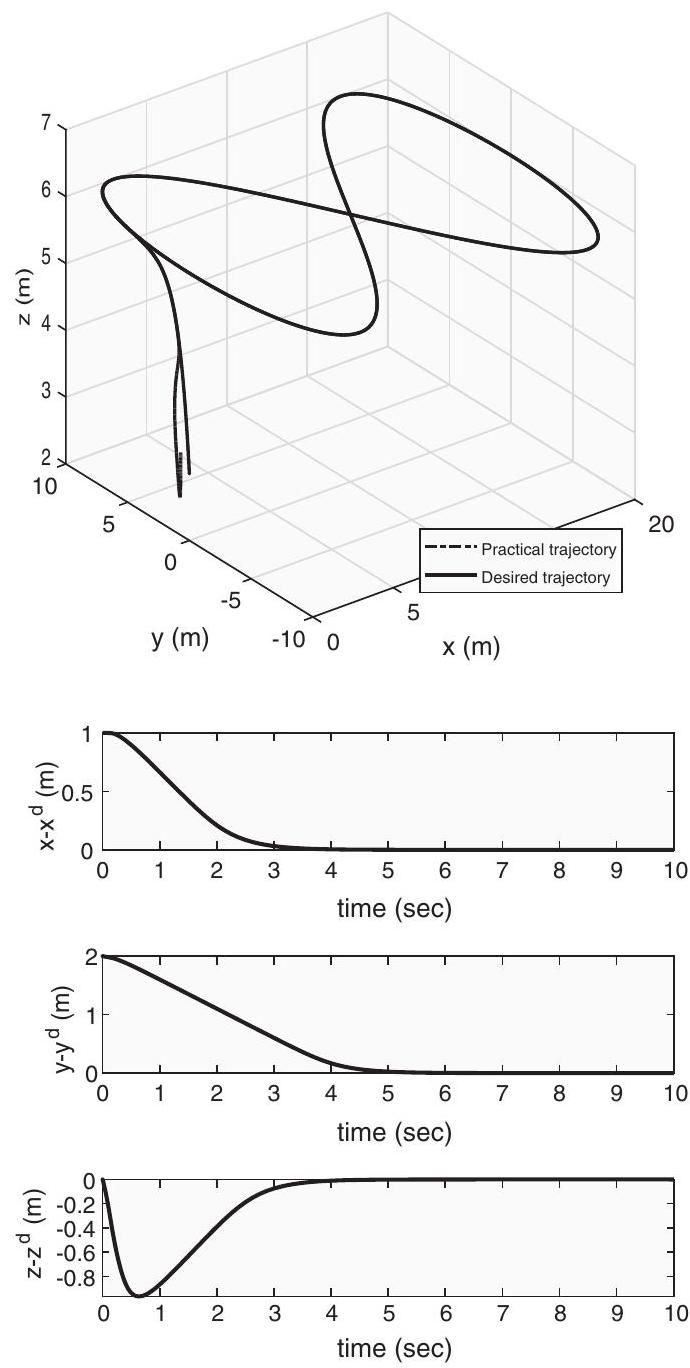
\includegraphics[max width=\textwidth, center]{2023_10_07_eefdf58cc80a47c1244eg-10}

F I G U R E 2 Position tracking in three-dimensional space

F I G U R E 3 Time response of $p-p^{d}$

\begin{center}
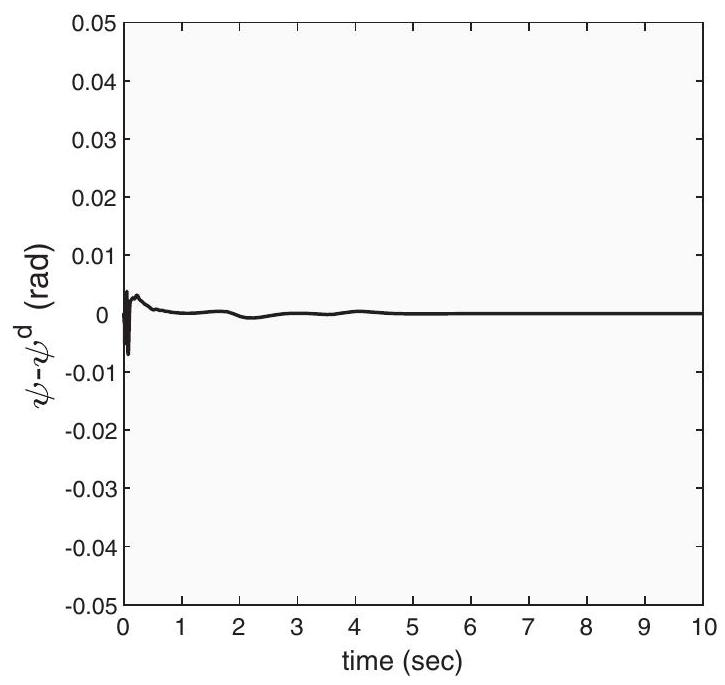
\includegraphics[max width=\textwidth]{2023_10_07_eefdf58cc80a47c1244eg-11(1)}
\end{center}

F I G U R E 4 Time response of $\psi-\psi^{d}$

\begin{center}
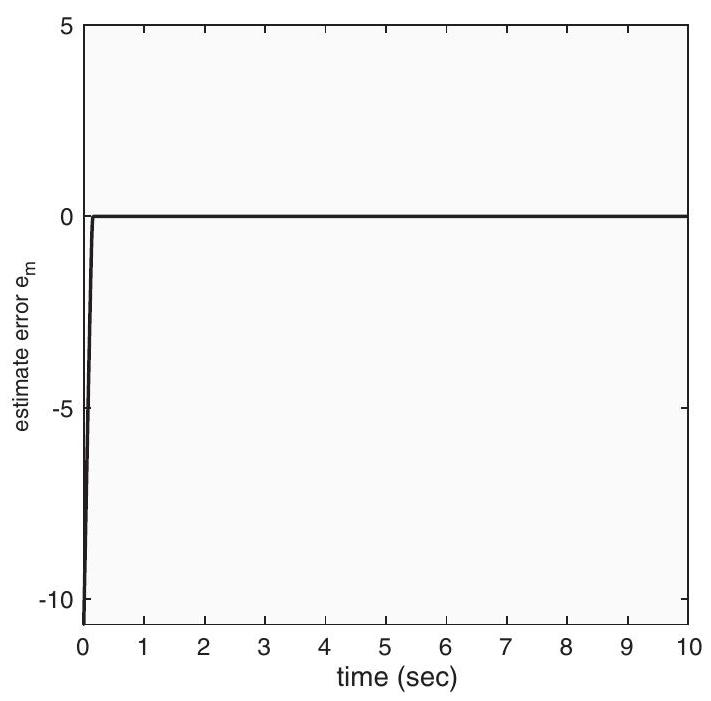
\includegraphics[max width=\textwidth]{2023_10_07_eefdf58cc80a47c1244eg-11}
\end{center}

F I G U RE 5 Time response of the estimate error $e_{m}$

\begin{center}
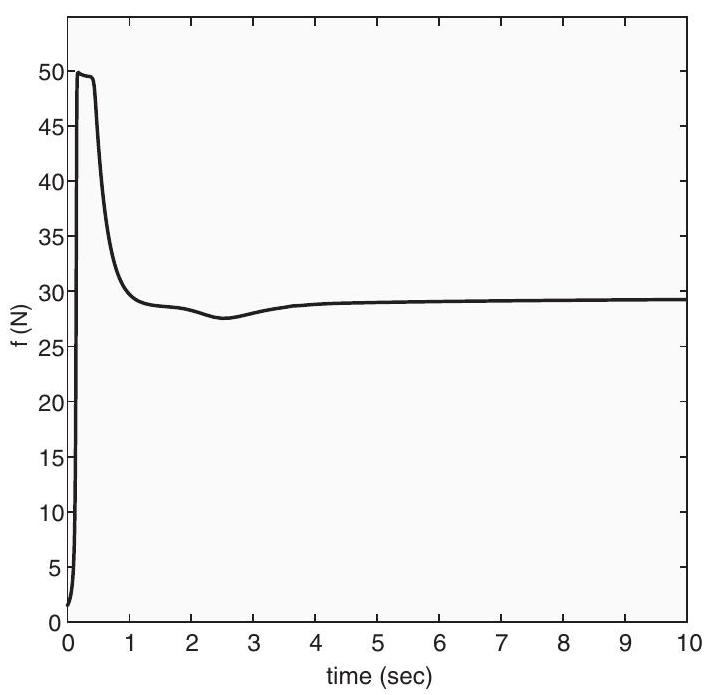
\includegraphics[max width=\textwidth]{2023_10_07_eefdf58cc80a47c1244eg-11(2)}
\end{center}

\begin{center}
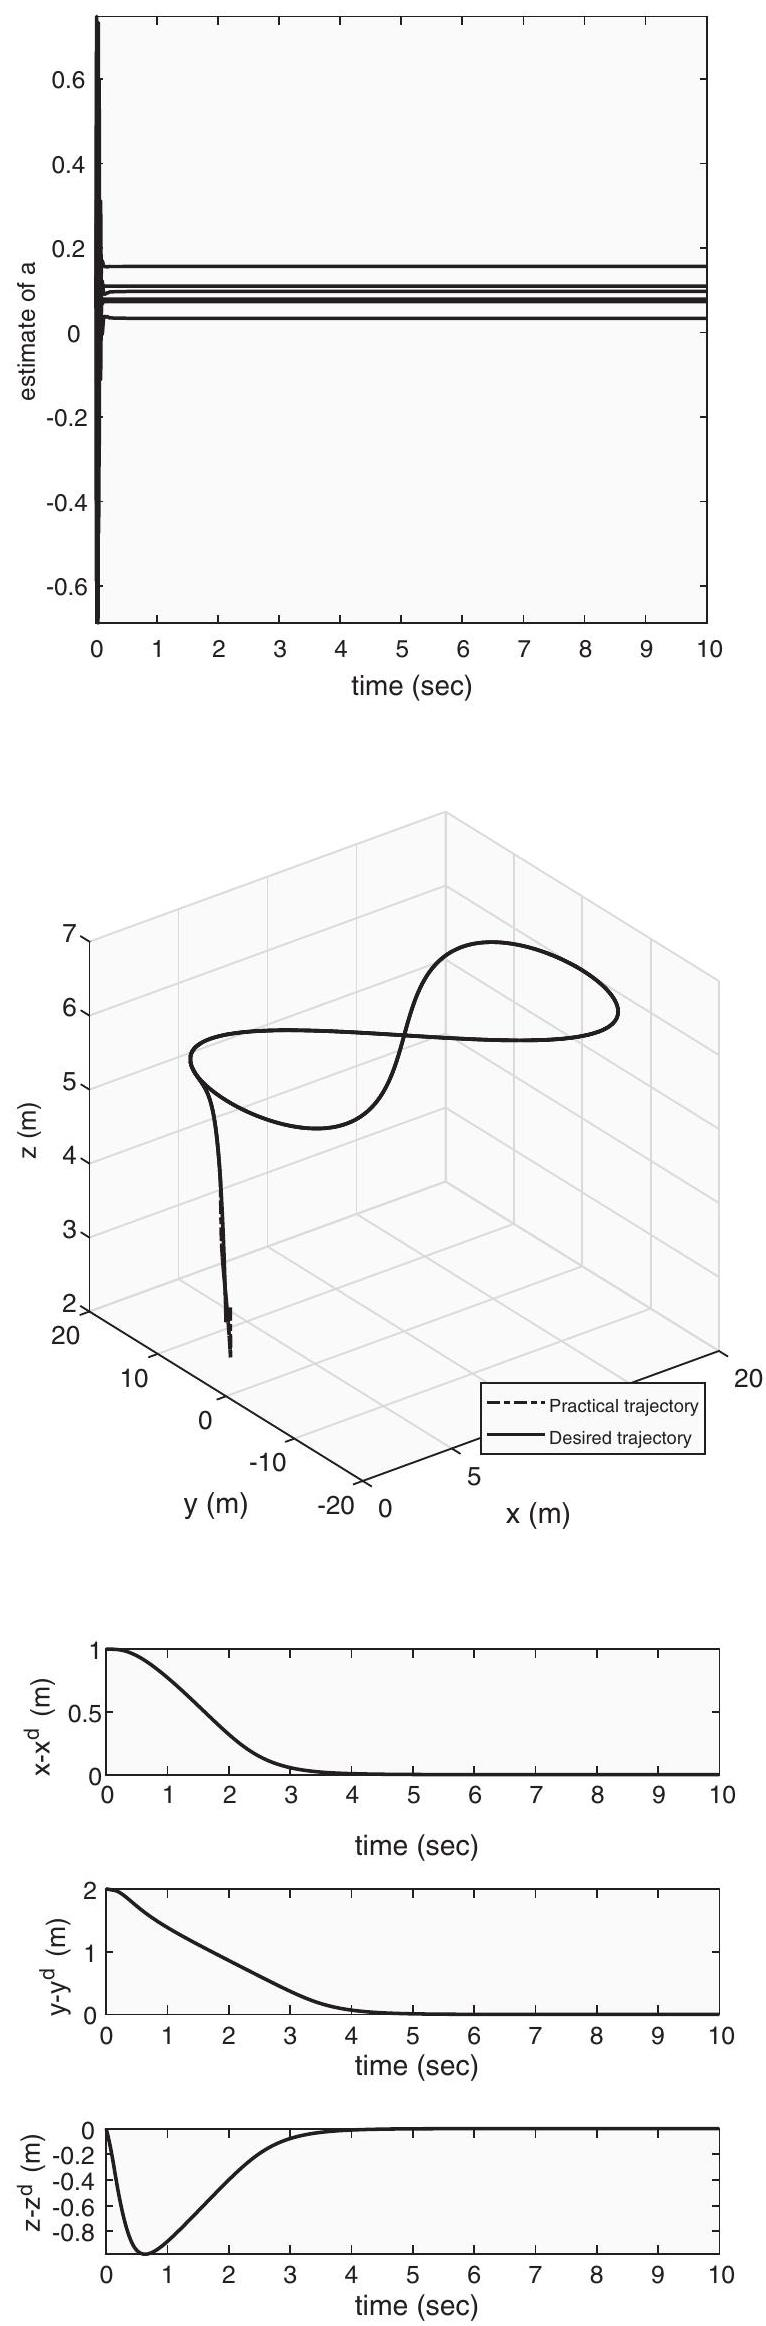
\includegraphics[max width=\textwidth]{2023_10_07_eefdf58cc80a47c1244eg-12}
\end{center}

F I G U R E 7 Time response of the estimate of $a$

F I G U R E 8 Position tracking in three-dimensional space F I G U R E 10 Time response of $\psi-\psi^{d}$

\begin{center}
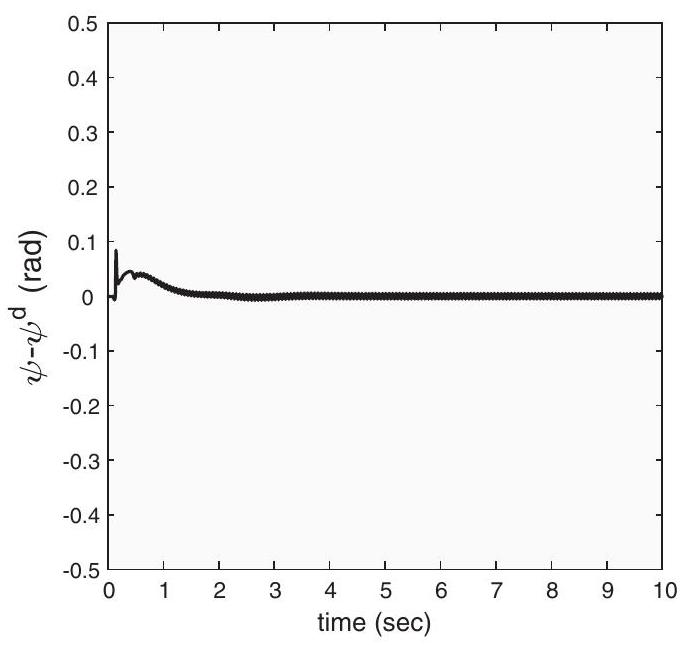
\includegraphics[max width=\textwidth]{2023_10_07_eefdf58cc80a47c1244eg-13(1)}
\end{center}

F I G U R E 11 Time response of the estimate error $e_{m}$

\begin{center}
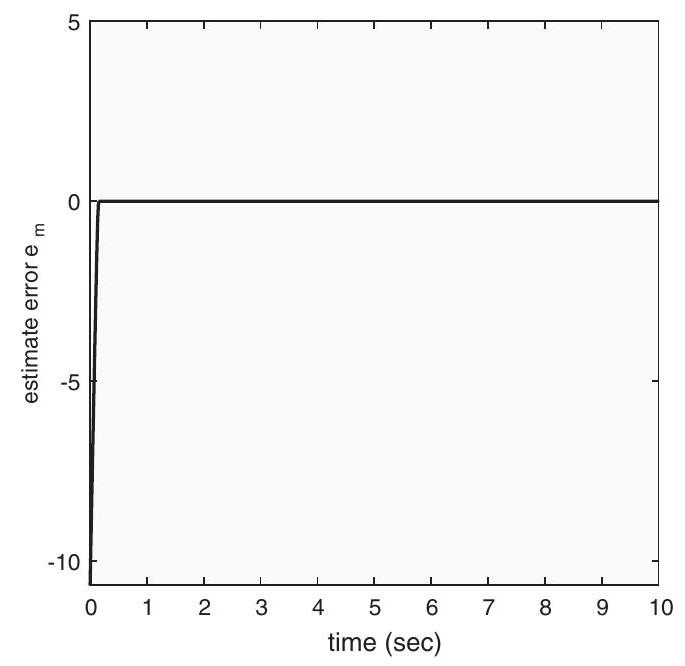
\includegraphics[max width=\textwidth]{2023_10_07_eefdf58cc80a47c1244eg-13}
\end{center}

F I G URE 12 Time response of $f$

\begin{center}
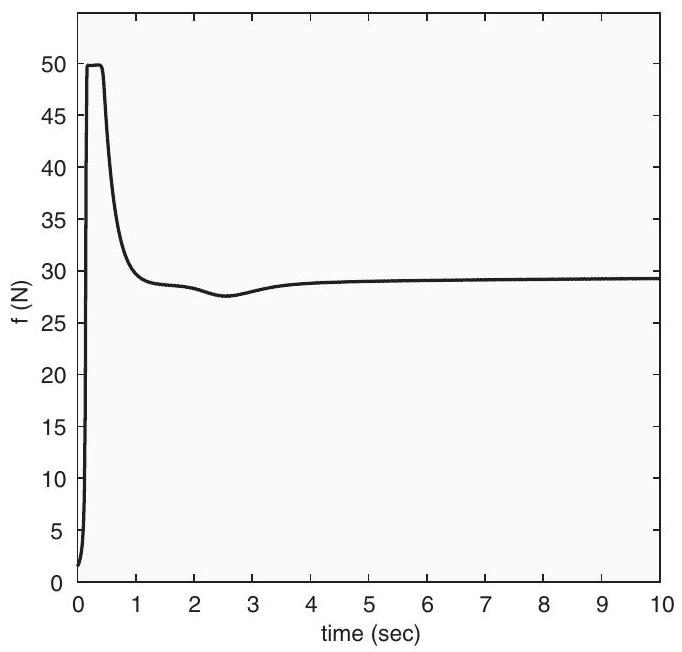
\includegraphics[max width=\textwidth]{2023_10_07_eefdf58cc80a47c1244eg-13(2)}
\end{center}

For the robust controller proposed in Theorem 2, simulations were also done with the same initial conditions. Figure 8 depicts the 3D position tracking. It shows that the position of the VTOL UAV asymptotically converges to its desired position $p^{d}$. The time response of the tracking errors of $x-x^{d}, y-y^{d}$, and $z-z^{d}$ are shown in Figure 9. Figure 10 depicts the response of $\psi-\psi^{d}$. It shows that $\psi$ asymptotically converges to its desired value. Figure 11 shows the estimate error $e_{m}$. It shows that the estimate error goes to zero. Figure 12 shows the total force $f$. It is shown that $f$ is always positive. The simulation results show the effectiveness of the robust controller in Theorem 2.

\section{I CONCLUSION}
This paper considered the tracking control problem of a quadrotor with parametric uncertainty. Adaptive and robust tracking controllers were proposed with the aid of the backstepping technique and the immersion and invariance technique. The proposed controllers ensure that the position of the system asymptotically converges to its desired trajectory and the Euler angle $\psi$ converges to its desired value. Furthermore, in the state feedback controllers the thrust force is guaranteed to be positive and the singularity of the Euler angles are avoided by a nonlinear transform in the controller design. Simulation results show the effectiveness of the proposed controllers.

\section{ORCID}
Wenjie Dong (1) \href{https://orcid.org/0000-0003-2842-1782}{https://orcid.org/0000-0003-2842-1782}

\section{REFERENCES}
\begin{enumerate}
  \item Zhao S, Dong W, Farrell JA. Quaternion-based trajectory tracking control of vtol-uavs using command filtered backstepping. Paper presented at: Proceedings of the 2013 American Control Conference; June 2013:1018-1023.

  \item Choi I-H, Bang H. Adaptive command filtered backstepping tracking controller design for quadrotor unmanned aerial vehicle. Proc Inst Mech Eng Part G J Aerosp Eng. 2011;226(04):483-497.

  \item Ha C, Zuo Z, Choi FB, Lee D. Passivity-based adaptive backstepping control of quadrotor-type uavs. Robot Autonom Syst. 2014;62(9):1305-1315. Intelligent Autonomous Systems.

  \item Zuo Z, Wang C. Adaptive trajectory tracking control of output constrained multi-rotors systems. IET Control Theory Appl. 2014;8(13):1163-1174.

  \item Wang L, Jia $\mathrm{H}$. The trajectory tracking problem of quadrotor UAV: global stability analysis and control design based on the cascade theory. Asian J Control. 2014;16(2):574-588.

  \item Lee T, Leok M, McClamroch NH. Geometric tracking control of a quadrotor uav on se(3). Paper presented at: Proceedings of the 49th IEEE Conference on Decision and Control (CDC); December 2010:5420-5425.

  \item Chaturvedi NA, Sanyal AK, McClamroch NH. Rigid-body attitude control. IEEE Control Syst Mag. 2011;31(3):30-51.

  \item Yu Y, Ding X. A global tracking controller for underactuated aerial vehicles: design, analysis, and experimental tests on quadrotor. IEEE/ASME Trans Mechatron. 2016;21(5):2499-2511.

  \item Lefeber E, van den Eijnden SJAM, Nijmeijer H. Almost global tracking control of a quadrotor UAV on se(3). Paper presented at: Proceedings of the 2017 IEEE 56th Annual Conference on Decision and Control (CDC); December 2017:1175-1180.

  \item Sun L, Zuo Z. Nonlinear adaptive trajectory tracking control for a quad-rotor with parametric uncertainty. Proc Inst Mech Eng Part G J Aerosp Eng. 2015;229(9):1709-1721.

  \item Zhao B, Xian B, Zhang Y, Zhang X. Nonlinear robust adaptive tracking control of a quadrotor UAV via immersion and invariance methodology. IEEE Trans Ind Electron. 2015;62(5):2891-2902.

  \item Hu J, Zhang $\mathrm{H}$. Immersion and invariance based command-filtered adaptive backstepping control of vtol vehicles. Automatica. 2013;49(7):2160-2167.

  \item Zhu B, Huo W. Adaptive backstepping control for a miniature autonomous helicopter. Paper presented at: Proceedings of the 201150 th IEEE Conference on Decision and Control and European Control Conference; December 2011:5413-5418.

  \item Zuo Z. Adaptive trajectory tracking control of a quadrotor unmanned aircraft. Paper presented at: Proceedings of the 30th Chinese Control Conference; July 2011:2435-2439.

  \item Teel AR. Global stabilization and restricted tracking for multiple integrators with bounded controls. Syst Control Lett. 1992;18(3):165-171.

  \item Farrell JA, Polycarpou M, Sharma M, Dong W. Command filtered backstepping. IEEE Trans Automat Control. 2009;54(6):1391-1395.

  \item Dong W, Farrell JA, Polycarpou MM, Djapic V, Sharma M. Command filtered adaptive backstepping. IEEE Trans Control Syst Technol. 2012;20(3):566-580.

  \item Ioannou P, Sun J. Robust Adaptive Control. Upper Saddle River, NJ: Prentice Hall Inc; 1996.

\end{enumerate}

How to cite this article: Dong W, Dony MN-A, Rafat M. Tracking control of vertical taking-off and landing vehicles with parametric uncertainty. Int J Adapt Control Signal Process. 2020;1-14.

\href{https://doi.org/10.1002/acs.3143}{https://doi.org/10.1002/acs.3143}


\end{document}